%!TEX root = ../thesis.tex
\documentclass[..thesis.tex]{subfiles}

\begin{document}
\TODO{First paragraph needs rewording and/or restructuring}
\TODO{Consider providing a stack trace in the appendices to illustrate what is the sample that we are gathering here}
Sampling profilers gather call traces from the observable program at regular intervals. Distribution of the gathered samples highlights the hotspots in the observable program. Higher frequency of a call trace suggests that more program's execution time was spent in that particular state. Profiling result is a statistical approximation of the program's performance. Thus, having more samples will provide a more accurate approximation. This approach also assumes that samples are gathered randomly as bias in the samples could potentially yield inaccurate results. 

Figure ~\ref{fig:samplingProf} on page ~\pageref{fig:samplingProf} helps to visualize the performance implications of the frequency of the gathered samples. The graph visualizes the performance outline of a simple program that executes two identical methods, \texttt{methodA} and \texttt{methodB}, alternately. This simple program executed for $911$ milliseconds during which $120$ usable samples were collected. $58$ of those samples contained \texttt{methodA} in its top call frame and $44$ contained \texttt{methodB} in its top frame.

Although sampling profiling does not provide precise time metrics for each method, it does provide a general overview to visualize the time spent in the profileable application's context. 

\begin{figure}[H]
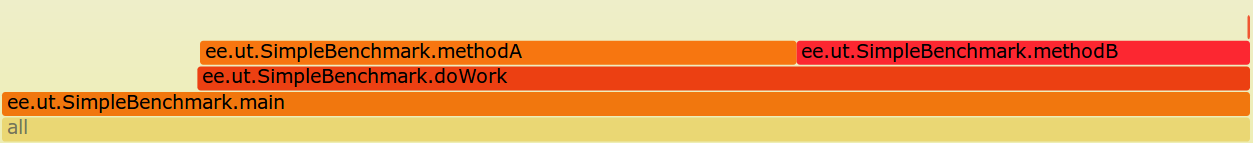
\includegraphics[scale=0.335]{samplingprofexample.png}
%\includegraphics[scale=0.6]{samplingprofexample2.png}
\caption{Visualization of sampling profiling output}
\label{fig:samplingProf}
\end{figure}
Due to the low amount of samples, it appears as \texttt{methodA} consumes more time than the \texttt{methodB} which is not the case in reality. Increasing the amount of call trace samples gathered could potentially draw a more accurate visualization of the program's performance.

\subsection{Sampling profiling challenges}
There are multiple problems that the implementations of the sampling profilers could experience. 
\subsubsection{Periodicity bias}
This problem occurs when the sampling interval catches on to some program's routine which executions match the sampling interval. Figure ~\ref{fig:periodicityBias} on page ~\pageref{fig:periodicityBias} illustrates the issue behing the bias. Suppose that the observable program runs \texttt{Method X} and \texttt{Method Y} alternatingly for some constant time period. If the dotted lines are the marks for the call trace samples taken during profiling, the results would be skewed as not a single sample represents \texttt{Method Y} in the results.

\begin{figure}[H]
\centering
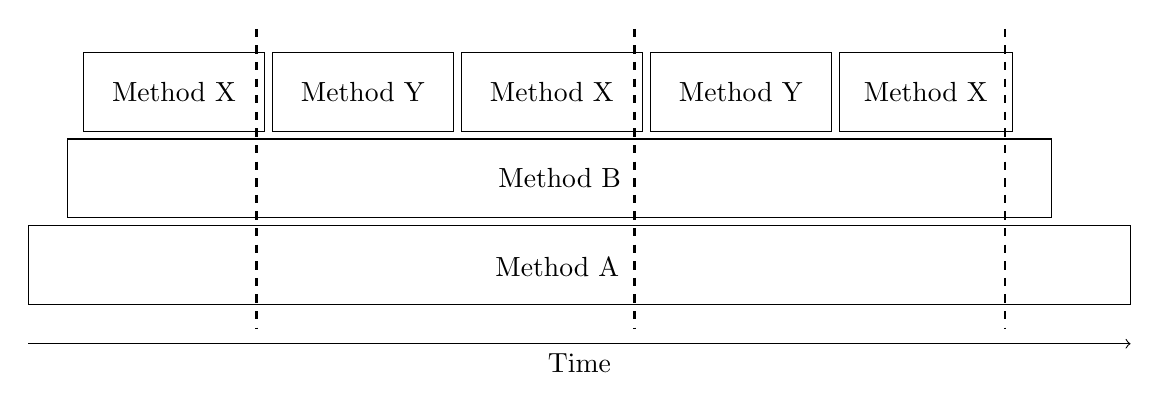
\begin{tikzpicture}
% Call stack rectangles
\draw (0,0) rectangle (14,1) node[pos=.48] {Method A};
\draw (0.5,1.1) rectangle (13,2.1) node[pos=.5] {Method B};
\draw (0.7,2.2) rectangle (3,3.2) node[pos=.5] {Method X};
\draw (3.1,2.2) rectangle (5.4,3.2) node[pos=.5] {Method Y};
\draw (5.5,2.2) rectangle (7.8,3.2) node[pos=.5] {Method X};
\draw (7.9,2.2) rectangle (10.2,3.2) node[pos=.5] {Method Y};
\draw (10.3,2.2) rectangle (12.5,3.2) node[pos=.5] {Method X};

% x-axis time arrow below
\draw[->] (0,-0.5) -- (14, -0.5) node[below, pos=.5] {Time};

% samples
\draw[dashed, thick] (2.9,3.5) -- (2.9,-0.3);
\draw[dashed, thick] (7.7,3.5) -- (7.7,-0.3);
\draw[dashed, thick] (12.4,3.5) -- (12.4,-0.3);

\end{tikzpicture}
\caption{Illustration of periodicity bias}
\label{fig:periodicityBias}
\end{figure}

\TODO{Ask supervisors whether it is acceptable to 'backreference' a figure shown previosuly in such manner.}
Real life example can be observed on the figure ~\ref{fig:samplingProf} on page ~\pageref{fig:samplingProf}. The sample application called two identical methods alternatingly after a constant interval or $4$ milliseconds without any mechanism to combat this periodicity bias. On the output graph, it can be observed that the \texttt{methodA} was present in a larger amount of samples than \texttt{methodB}. In reality, it would be expected for \texttt{methodA} and \texttt{methodB} to have approximately the same number of call trace samples representing them.

Possible ways to tackle this problem would be to randomize the sampling interval by having a random number of time units offseting the sampling interval. 
\subsubsection{Safepoint bias}
Sampling profiling assumes that the obtained samples are acquired randomly. When gathering samples from a program running on the Java Virtual Machine, one must take \textit{safepoints} into consideration. 

\TODO{subsubsubsections for safepoint definition and demonstration?}

Safepoints in the Java Virtual Machine are defined as points during the program's execution during which all of the threads are in a consistent and well known state. Safepoints are necessary for various Java Virtual Machine's operations such as the garbage collection, method deoptimization and class redefinition. \cite{hotspot_glossary}

 
It has been shown that most of the existing Java profilers require the Java Virtual Machine to be stopped on a safepoint in order to obtain the call trace sample from the profileable thread. However, this mechanism also casts a shadow on the profling results as this implies that the samples are not aquired randomly but rather require the Java Virtual Machine to be in a specific state. \cite{mytkowicz_evaluating_2010}

The execution of the code sample in listing ~\ref{lst:safepoint} illustrates this issue well. 
\begin{lstlisting}[language=java,style=def,label={lst:safepoint}, caption={Counted loops do not contain safepoints}]
int k = 0;
for (int i = 0; i < Integer.MAX_VALUE; i++) {
	for (int j = 0; j < 2; j++) {
    	k++;
    	if ((k % 2) == 1) k++;
	}
}
\end{lstlisting}
As various Java Virtual Machine routines are nondeterministic, it is impossible to predict when does the Java Virtual Machine signal its threads to be stopped on a safepoint. However, if such request should occur in the middle of the counted loop's execution in listing ~\ref{lst:safepoint}, the thread executing the loop's instructions will not stop until the loop has finished. Thus, if an ordinary profiler signals the thread for a call trace sample, it is delayed until the thread executing the loop's instructions finishes its job. 

To measure the actual time that is spent waiting for the Java Virtual Machine to stop all its threads on a safepoint, \texttt{-XX:+PrintGCApplicationStoppedTime} flag can be used to measure this metric. This flag outputs the time it takes for the Java Virtual Machine to stop all threads in order to execute its subroutine and the time that this operation took in total. Due to nondeterminicity, the sample code in listing ~\ref{lst:safepoint} was executed $100$ times. The worst case among $100$ program runs recorded a Java Virtual Machine operation that took $7.5171863$ seconds and $7.5171122$ seconds of that time was spent on stopping the thread. It is worth mentioning that $11.5181148$ seconds was spent on the whole execution of that particular attempt.

\TODO{Explain that it's bad, mkay?}


Such bias during obtaining the call trace clearly contradicts the randomness prerequisite for sampling profiling.




\TODO{Ideas to expand on:}
Nitsan Wakart on safepoints not present in indexed loops: The reason it's so stuck is because the computation is running in a 'counted' loop, and counted loops are considered short by the JVM. Short enough to not have safepoints. This thread refusing to come to a safepoint will lead to all other threads suspending indefinitely at the next safepoint operation.


Safepoints are not precisely documented in the language specifications as they are implementation details of the JVM and each JVM implementation may interpret safepoints differently but they generally work in a similar manner.

JVM raises a flag to notify threads to stop on safepoint and then waits the threads to stop on a safepoint. Thread polls for safepoint flag after every 2 bytecode instructions (when in interpreter), end of non-counted loop, method exit, JNI call exit(C1/C2 compiled code)

\subsubsection{Observer effect}
\TODO{Introducing overhead whilst profiling could have implications on the results: http://www.inf.usi.ch/faculty/hauswirth/publications/pldi10.pdf}

\subsection{Sampling profiling possible implementations for the JVM}



\subsubsection{\texttt{AsyncGetCallTrace} profilers}
These kind of profilers make use of an undocumented JVM method \texttt{Async\-Get\-Call\-Trace} \cite{agct_source} which enables obtaining call traces from a thread without the safepoint bias. Due to this characteristic, profiling samples tend to be more 'honest' since the JVM does not have to stop on a safepoint in order to obtain the call trace of the running thread.

Notable examples of such profilers are Honest Profiler and Java Mission Control. \TODO{Citation needed}


Points to expand on:
\begin{enumerate}
	\item Sends interrupt signal to thread and then runs signal handler to collect the stack trace. Only interrupted thread is stopped.
	\item Does not require the thread to be stopped on a safepoint.
	\item Shows only Java stack. (Most problems can be solved on Java level - Nitsan Wakart)
	\item Only operations on CPU are sampled. Blocking/concurrency issues won't be spotted.
\end{enumerate}

\TODO{Pros and cons}


\subsubsection{\texttt{GetStackTrace} profilers}
This method uses function from the official JVM Tooling Interface API \cite{jvmti_doc} called \texttt{GetStackTrace}.

Some points to expand on:
\begin{enumerate}
	\item Safepoint biased. Requires all the threads to be stopped on a safepoint in order top collect call traces
	\item Has higher overhead when compared to other methods. Application having many threads might take a long time for all the threads to reach a safepoint.
\end{enumerate}

\subsubsection{Native profilers}
\subsubsection{\texttt{jstack}}



\end{document}